% Chapter 1

\chapter{Introducción} % Main chapter title
\label{Chapter1} % For referencing the chapter elsewhere, use \ref{Chapter1} 

%----------------------------------------------------------------------------------------

% Define some commands to keep the formatting separated from the content 
\newcommand{\keyword}[1]{\textbf{#1}}
\newcommand{\tabhead}[1]{\textbf{#1}}
\newcommand{\code}[1]{\texttt{#1}}
\newcommand{\file}[1]{\texttt{\bfseries#1}}
\newcommand{\option}[1]{\texttt{\itshape#1}}
%----------------------------------------------------------------------------------------

En 1850 se creía que el Cólera, una enfermedad intestinal contagiosa y mortal,
era propagado por aire. Esta creencia se refutó en 1854 cuando un médico
inglés, John Snow, dibujó en un mapa todos los casos de contagio ocurridos en
el \textit{Soho} de Londres (figura \ref{snow_map}). El mapa mostraba que la
mayoría de casos ocurrían en las cercanías de un pozo de agua específico. La
epidemia cesó cuando, por recomendación de Snow, se cerró este pozo
\parencite{snow}.

\begin{figure}
  \caption{Mapa que muestra casos de contagio del Cólera, representando cada contagio con una barra en el edificio donde se produjo.}
\label{snow_map}
  \makebox[\textwidth]{
  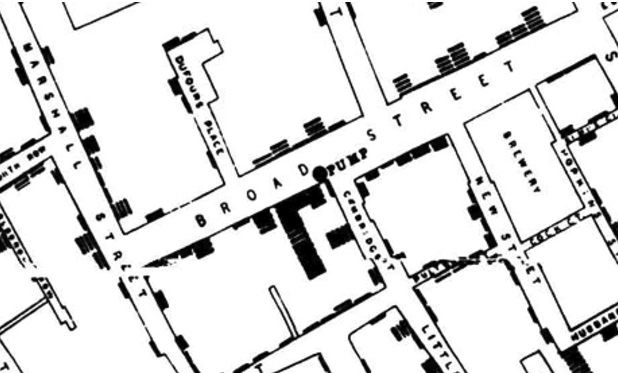
\includegraphics[width=0.7\linewidth]{snow_map}
  }
\end{figure}

Este es uno de los primeros ejemplos de un problema resuelto gracias al
análisis de datos. Una de las ventajas de las nuevas tecnologías es la gran
cantidad de datos que son capaces de generar para problemas específicos. Esto
abre nuevas posibilidades para resolver problemas que antes eran impensables.
Sin embargo, de la misma manera que alguien tuvo que pintar todos esos puntos
en el mapa de John Snow, los datos deben ser tratados para poder extraer
conocimiento de ellos. 

Una gran cantidad de datos requiere una gran cantidad de recursos humanos para
extraer conocimiento, sobre todo cuando los datos son tan complejos
como reconocer una voz en un fichero de audio, entender la intención de un
texto o detectar un objeto en una imagen.

\section{Aprendizaje automático}

El aprendizaje automático es un campo de las ciencias de la computación
cuyo objetivo es crear sistemas que sean capaces de realizar determinadas
tareas mejorando mediante la experiencia, sin necesitar que se le diga
explícitamente como realizarlas \parencite{mitchell}.

Usando este tipo de sistemas es posible enseñar a una máquina a extraer
conocimiento de diferentes datos si es capaz de ver ejemplos anteriores.
Por ejemplo, puede ser capaz de reconocer peces en una imagen si se le 
provee de ejemplos resueltos.

Conseguir sistemas de este tipo hace que se puedan resolver problemas
cuya solución no estaba al alcance de nadie que no tuviese grandes
cantidades de recursos.

\section{\textit{Kaggle}}

En el año 2007, \textit{Netflix} creó una competición para mejorar su motor de
recomendación de películas. Publicó un conjunto de datos con las películas
elegidas por los diferentes usuarios y pidió a los participantes realizar un
modelo predictivo usando este conjunto de datos. Evaluaron los modelos
predictivos presentados usando un conjunto de datos diferente y otorgaron el
premio al que menos error presentaba. El premio para el mejor modelo predictivo
era de un millón de dólares.

En 2010 el economista australiano Anthony Goldbloom, inspirándose en la idea de
la competición de \textit{Netflix}, creó \textit{Kaggle}. Esta es una
plataforma de competiciones de análisis y modelización predictiva de datos.

La plataforma funciona de la siguiente manera: un equipo promotor
contacta con \textit{Kaggle} y prepara un conjunto de datos para la competición.
Un subconjunto de esos datos son publicados en la web para el uso de los
participantes. El otro subconjunto, oculto, se usa para determinar el mejor
modelo presentado y declarar un ganador.

El conjunto de datos presentado contiene las respuestas de cada elemento
(permitiendo así que los modelos usen aprendizaje supervisado). Junto a los
datos se especifica una métrica que servirá para medir la bondad del modelo.

Para presentar el modelo el participante debe presentar las predicciones del
conjunto de test en la web de \textit{Kaggle}. La puntuación obtenida según la
métrica sobre una parte del conjunto de test se hará pública en la tabla de
posiciones pública. Cuando la competición termina se genera una tabla de
posiciones privada, donde se publica la puntuación del modelo usando el
conjunto de test completo y es con esta puntuación con la que se determina el
ganador. Se hace de esta manera para evitar que los participantes sobreajusten
el modelo al conjunto de test.

Existen varios tipos de competiciones a las que los usuarios se pueden
presentar:

\begin{itemize}
  \item \textit{\textbf{Getting started}}: Competiciones sencillas organizadas por la
      misma plataforma con la finalidad de que los usuarios se familiaricen con
      los modelos predictivos y la estructura de las competiciones. Suelen tener
      un conjunto de datos ordenado y sencillo, y existe mucha documentación y
      ayuda en los foros.
  \item \textit{\textbf{Playground}}: Competiciones que no resuelven problemas
      reales, diseñadas para que los usuarios experimenten y prueben diferentes
      ideas. No tienen ningún premio.
  \item \textit{\textbf{Research}}: El objetivo de estas competiciones es la
      investigación sobre diferentes técnicas o de problemas de bien común.
      Muchas de estas competiciones tienen como premio la invitación a
      conferencias o a publicar los resultados en algún medio. Suelen requerir
      que las soluciones sean publicadas como código abierto.
  \item \textit{\textbf{Recruiting}}: Los organizadores de estas competiciones
      buscan contratar a los mejores participantes.
  \item \textit{\textbf{Featured}}: Las competiciones con más dificultad y
      mejores premios. Buscan resolver un problema real y posiblemente
      comercial. Aquí entraría la competición de \textit{Netflix}.
\end{itemize}

A principios de 2017 \textit{Kaggle} fue comprado por \textit{Google}, aunque por ahora sigue siendo una
plataforma independiente funcionando bajo su propio nombre.

\section{Reconocimiento de imágenes}

Uno de los granes problemas dentro del aprendizaje automático es
el reconocimiento de objetos en imágenes. Detectar diferentes 
objetos y situaciones de una imágen tal y como lo hace un humano
permitiría automatizar muchísimos procesos, desde la conducción
autónoma hasta la digitalización de libros.

El desarrollo de redes neuronales convolucionales en arquitecturas de
aprendizaje profundo está consiguiendo precisiones similares a la humana en
problemas de reconocimiento visual \parencite{taigman}. Esto hace que sea cada
vez más interesante aplicar este tipo de soluciones a problemas de
clasificación visual donde antes no era posible.

\section{Reconocimiento de imágenes}

La competición de \textit{Kaggle} que se quiere resolver aquí tiene como
objetivo clasificar peces dentro de imágenes de barcos pesqueros. Esto
permitirá en un futuro predecir patrones migratorios, estudiar patrones de
pesqua o vigilar que la pesca sea una actividad que no dañe al medio ambiente.
Sin embargo es necesario encontrar un sistema que permita distinguir diferentes
peces tal y como lo haría un humano.

En este trabajo se intentarán aplicar técnicas de aprendizaje profundo para
resolver este problema, variando arquitecturas y usando redes preentrenadas. 

